
\subsection{Numerical setup}

Validation study is performed in order to study the influence of domain truncation on the LES of flow around sections. The numerical setup is described in detail earlier in section 2 and the setup for the domain validation simulations follows a very similar approach. The airfoil used for the study is ED36F128 designed at the Aeronautics and Vehicle Engineering department at KTH, Stockholm, where several experiments have been performed for both static \citep{lokatt17} and dynamic flow cases \citep{lokattthesis}. The chord-based Reynolds number used in the investigation is $Re_{c}=100,000$ and the angle of attack is set to $\alpha=6.7^{\circ}$. The spanwise width of the domain for all simulations was set to $l_{z}/c=0.1$. The flow is tripped to induce flow transition on both the suction and pressure side of the airfoil at a chord-wise location of $x/c=0.1$. Data from a RANS simulations with the $k$-$\omega$ SST turbulence model is used to obtain the velocity field and the kolmogorov length scale $\eta$. The RANS velocity field data is imposed as Dirichlet boundary condition on the inlet and far-filed boundaries. Periodic boundary conditions are applied on the spanwise boundaries of the domain. Simulations are performed using Nek5000 \citep{nek5000} with an $11^{th}$ order polynomial discretization. Velocity and length scales are normalized by free-stream velocity and chord length respectively. The grid resolution in the boundary layer around the airfoil is set such that $\Delta x^{+}\approx18$, $\Delta y_{w}^{+}\approx0.6$, $\Delta z^{+}\approx 9$. In order to account for the varying shear-stress values over the airfoil the following rules are used for the determination of the resolution:
\begin{enumerate}[topsep=5pt]
	\item The $u_{\tau}$ values from the RANS are used without modification in the region $0.1\le x/c\le0.6$ for both the pressure (ps) and suction sides (ss).
	\item For $x/c>0.6$, the $u_{\tau}$ from the pressure-side was used to design the mesh on both the suction and the pressure sides. The strong adverse-pressure gradient on the suction-side causes flow separation and $u_{\tau}\approx0$. Thus the pressure-side is used to design the mesh on both sides.
	\item For $x/c<0.1$, a constant $u_{\tau}$ value was used which was equal to the value at $x/c=0.1$ for both the suction and pressure sides.
	\item The spectral-element distribution is uniform in the span-wise direction with the value of $u_{\tau}$ at $x/c=0.25$ used for calculating the $\Delta z^{+}$ spacing.
	\item In the wake the criteria is based on the kolmogorov length scale $\eta$. The resolution in the wake is set such that $\Delta x,\Delta y,\Delta z\le10\eta$. The value of $\eta$ is estimated from the RANS solution. 
\end{enumerate}

\subsection{Validation cases}

Table~\ref{table:validation_cases} lists the different domain sizes tested in the present investigation along with the boundary condition used at the outlet boundary of the domain. All distances are measured from the leading-edge. All computational domains contain a curved inflow due to the C-grid type mesh topology. Thus the inlet distance is a radial distance from the leading-edge. A large reference case is set up in order to compare the results of the simulations with domain truncation. The stress-free boundary condition is used at the outlet for the reference case. In the subsequent test cases the energy-stabilizied outflow boundary condition as suggested by \cite{dong2014} is used. The boundary condition has been shown to improve accuracy and numerical stability in severely truncated domains \citep{dong2014}. 
\begin{table}[h]
	\centering
	\begin{tabular}{llllll}
		No. & Case Name	& Inlet & Far-field & Outlet & Outlet B.C. \\
		\hline
		\hline
		1 & Reference	& $5c$ & $5c$ & $5c$ & Stress-free \\
		2 & FF1W3	& $1c$ & $1c$ & $3c$ & Dong \\
		3 & FF2W4	& $2c$ & $2c$ & $4c$ & Dong
	\end{tabular}
	\vspace{5pt}
	\caption{Validation cases}
	\label{table:validation_cases}	
\end{table}
A 2-D cross-section of the grid for the reference domain is visualized in figure~\ref{fig:domain_grid_reference}. Iso-contours of the instantaneous vortical structures in the flow-field for the reference case are depicted in figure~\ref{fig:la2_reference}. All simulations are run for $20$ simulation time units and all statistics from the first $10$ time units are discarded to remove initial transient effects.
\begin{figure}[h]
	\centering
	\begin{subfigure}[b]{0.49\textwidth}
		\centering
		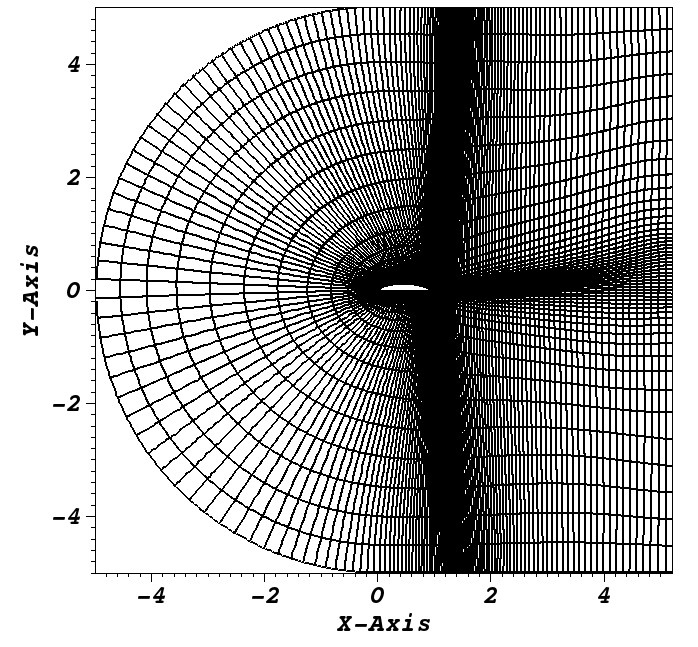
\includegraphics[width=1.0\columnwidth]{domain_reference}
		\caption{}
		\label{fig:domain_reference}
	\end{subfigure}
	\begin{subfigure}[b]{0.49\textwidth}
		\centering
		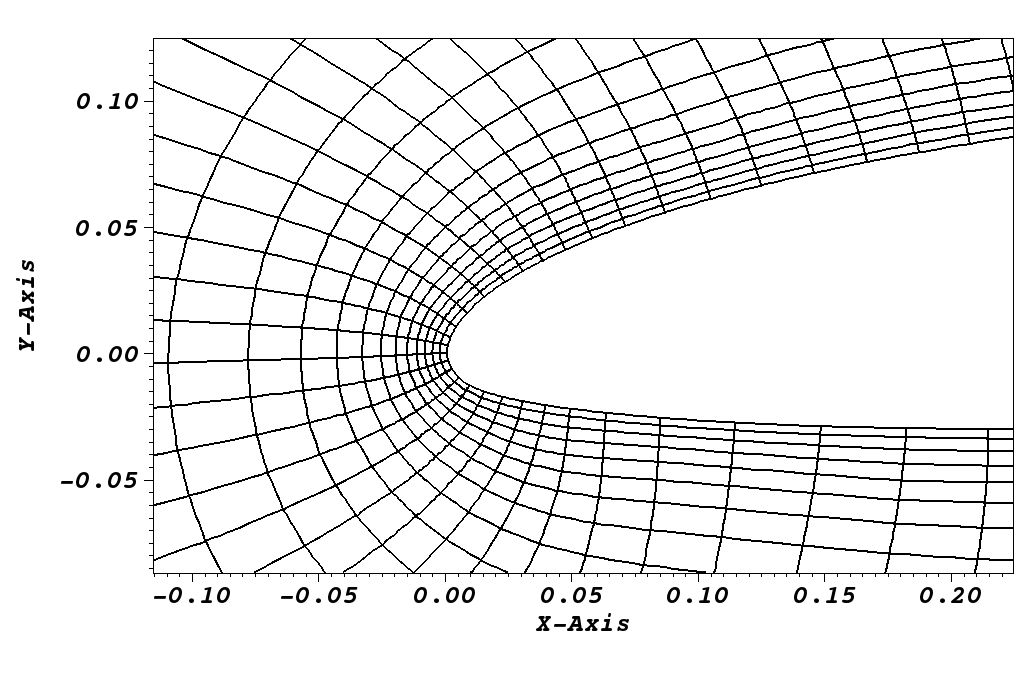
\includegraphics[width=1.0\columnwidth]{grid_reference}
		\caption{}
		\label{fig:grid_reference}
	\end{subfigure}
	\vspace{10pt}
	\caption{The simulation domain (a) and a close-up (b) near the leading edge, of the orthogonal and structured spectral-element grid for the reference case.}
	\label{fig:domain_grid_reference}
\end{figure}

\begin{figure}[h]
	\centering
	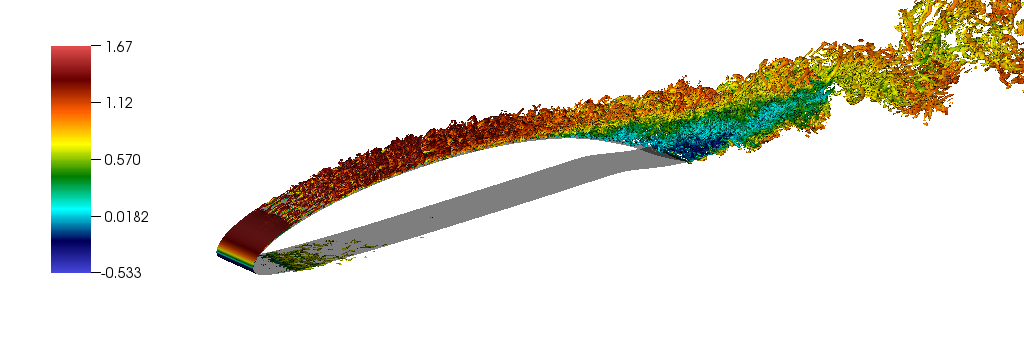
\includegraphics[width=0.9\textwidth,height=0.35\textwidth]{la2_reference.png}
	\caption{Visualization of the instantaneous flow structures identified by the $\lambda_{2}$ criterion \cite{jeong95}. The isocontours are colored by streamwise velocity.}
	\label{fig:la2_reference}
\end{figure}

In the case FF1W3 the domain is truncated such that the far-field and inlet boundaries are one chord away from the airfoil ($FF=1$) and the wake region is truncated to three chords downstream of the leading-edge ($W=3$). Comparison of the wall-shear stress with the Reference case is shown in figure~\ref{fig:outflow_ff1w3}. Even with such a severely truncated computational domain, it is found that the flow field is only marginally disturbed with respect to the Reference case. The wall shear-stress ($\tau_{w}$) deviates only slightly from the reference values and this deviation occurs near a local peak of $\tau_{w}$ at $x/c\approx0.24$.
%% FF1 W2
\begin{figure}
	\centering
	\begin{subfigure}[h]{0.49\textwidth}
		\centering
		\caption{}		
		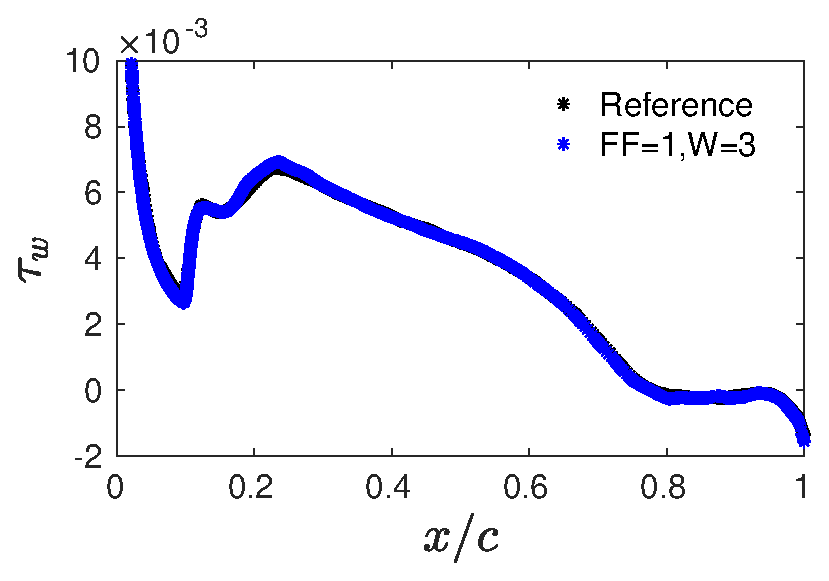
\includegraphics[width=0.9\columnwidth]{outflow_ff1w2_tauw}
		\label{fig:outflow_ff1w2_ws}
	\end{subfigure}
	\begin{subfigure}[h]{0.49\textwidth}
		\centering
		\caption{}		
		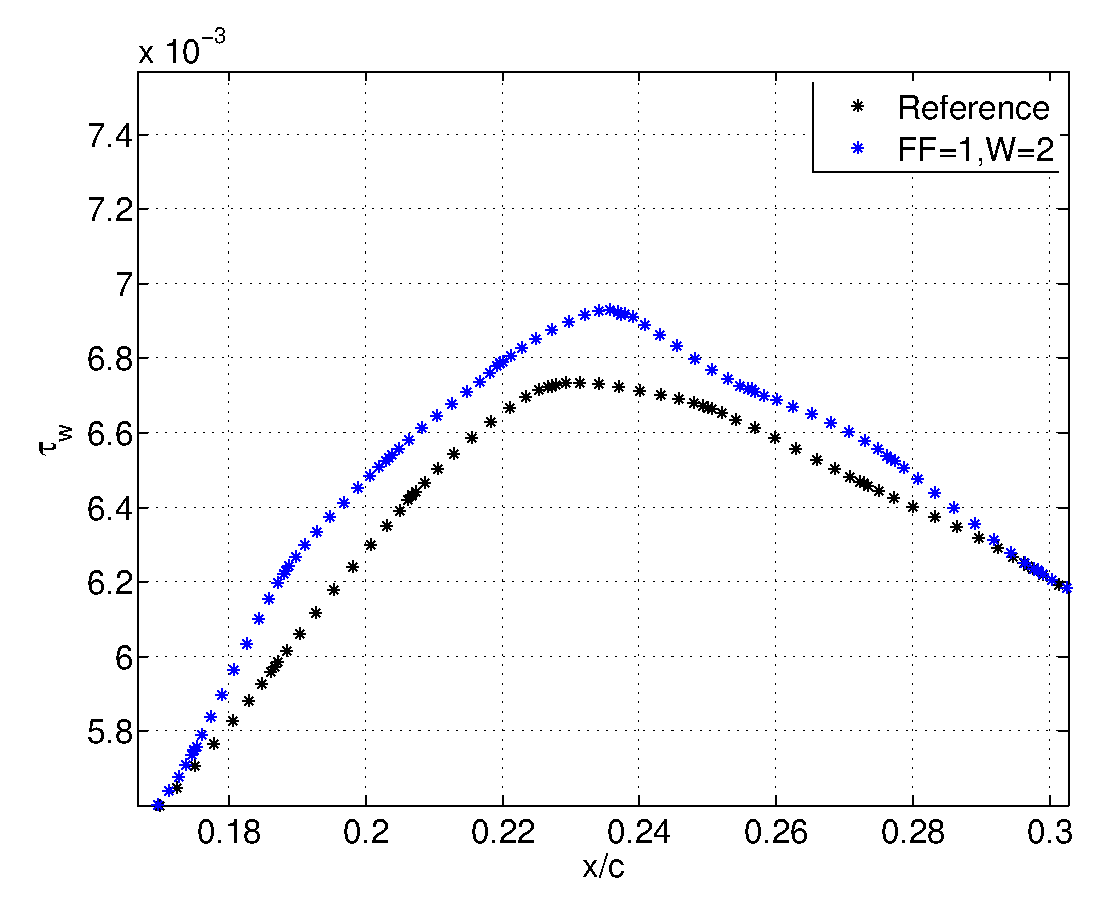
\includegraphics[width=0.9\columnwidth]{outflow_ff1w2_tauw_close}
		\label{fig:outflow_ff1w2_ws_close}
	\end{subfigure}
	\caption{The suction-side wall shear-stress comparison for the case FF1W3 depicting (a)the  chord-wise variation of $\tau_{w}$ and (b) the close-up region near the peak of the wall shear-stress.}
	\label{fig:outflow_ff1w3}
\end{figure}

For the case FF2W4 the domain size is slightly increased such that the far-field is now two chords away ($FF=2$) and the wake region is truncated to four chords downstream of the leading-edge ($W=4$). The deviation of wall shear-stress nearly vanishes. Figure~\ref{fig:outflow_ff2w3_ws} shows the development of $\tau_{w}$ across the airfoil which matches well with the reference case, and figure~\ref{fig:outflow_ff2w3_ws_close} shows the close-up region near the peak $\tau_{w}$ where, unlike figure~\ref{fig:outflow_ff1w2_ws_close}, no large deviation from the reference case values is visible.
\begin{figure}
	\centering
	\begin{subfigure}[h]{0.49\textwidth}
		\centering
		\caption{}		
		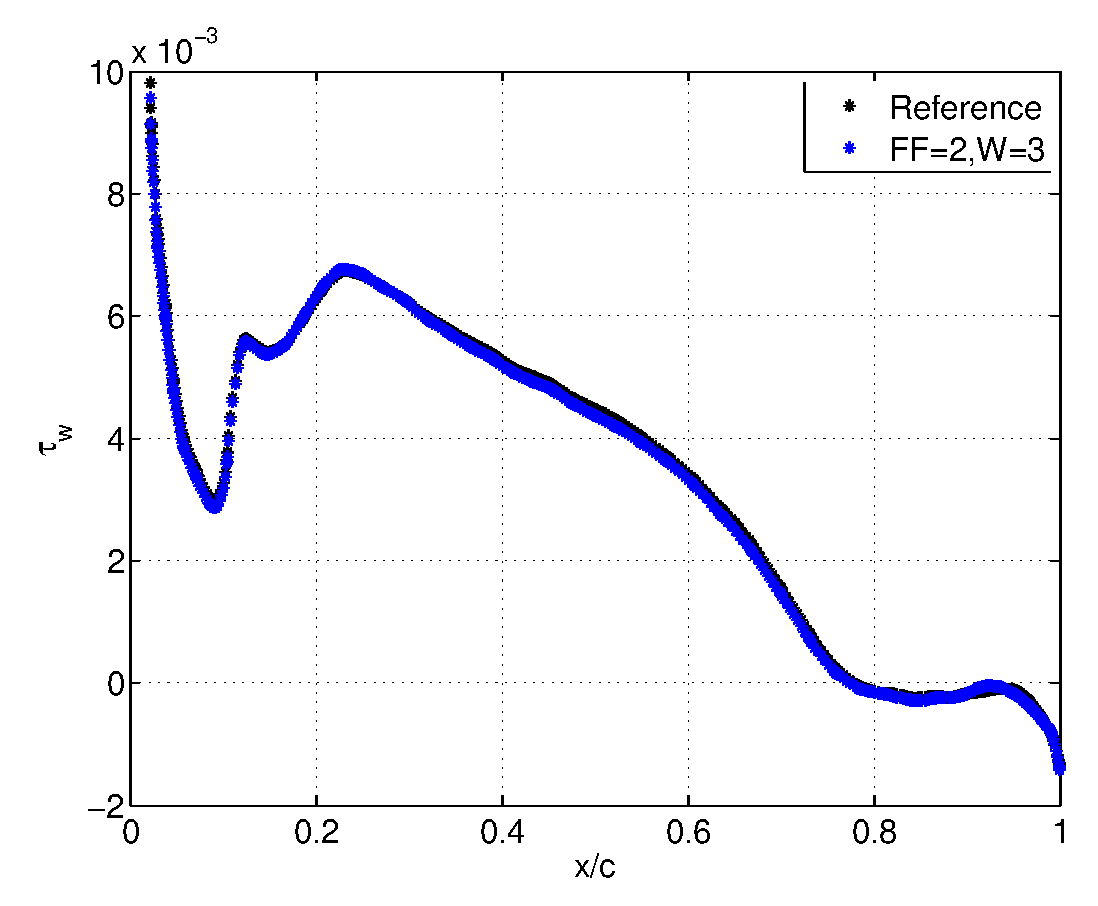
\includegraphics[width=0.9\columnwidth]{outflow_ff2w3_tauw}
		\label{fig:outflow_ff2w3_ws}
	\end{subfigure}
	\begin{subfigure}[h]{0.49\textwidth}
		\centering
		\caption{}		
		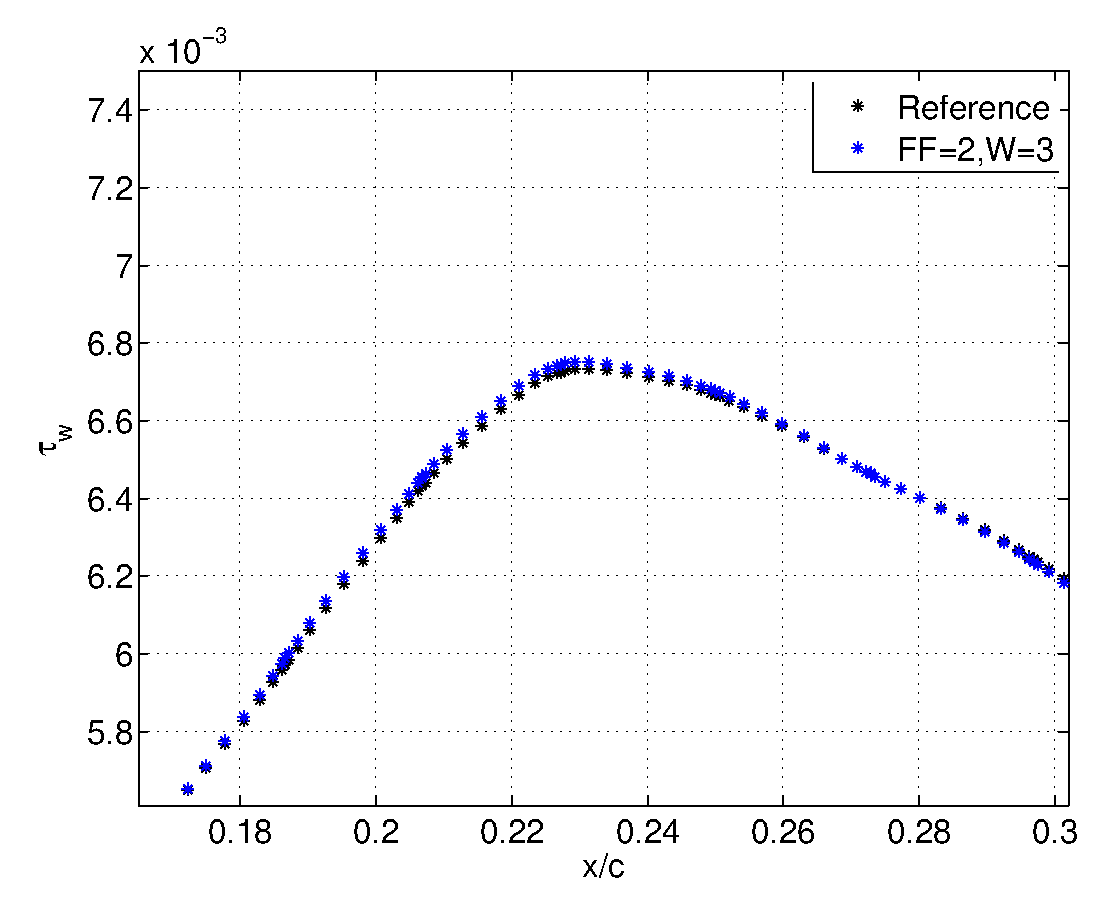
\includegraphics[width=0.9\columnwidth]{outflow_ff2w3_tauw_close}
		\label{fig:outflow_ff2w3_ws_close}
	\end{subfigure}
	\caption{The suction-side wall shear-stress comparison for the case FF2W4 depicting (a)the  chord-wise variation of $\tau_{w}$ and (b) the close-up region near the peak of the wall shear-stress.}
	\label{fig:outflow_ff2w3}
\end{figure}
Mean flow profiles (figure~\ref{fig:outflow_ff2w3_up}) and Reynolds stress terms ($\ref{fig:outflow_ff2w3_rs}$), evaluated at $x/c=0.6$ on the suction side, are examined for this case. All the evaluated quantities show a good agreement with the reference case values. Furthermore, mean velocity profile is evaluated in the separated region at $x/c=0.85$ and even in the separated region a very good agreement is found as evident in figure~\ref{fig:outflow_ff2w3_meanu_sep}. In the separated region $\tau_{w}$ is nearly zero, therefore the mean velocity is normalized using the far-field velocity of $U_{\infty}=1.0$.
%% FF2 W3
\begin{figure}
	\centering
	\begin{subfigure}[h]{0.49\textwidth}
		\centering
		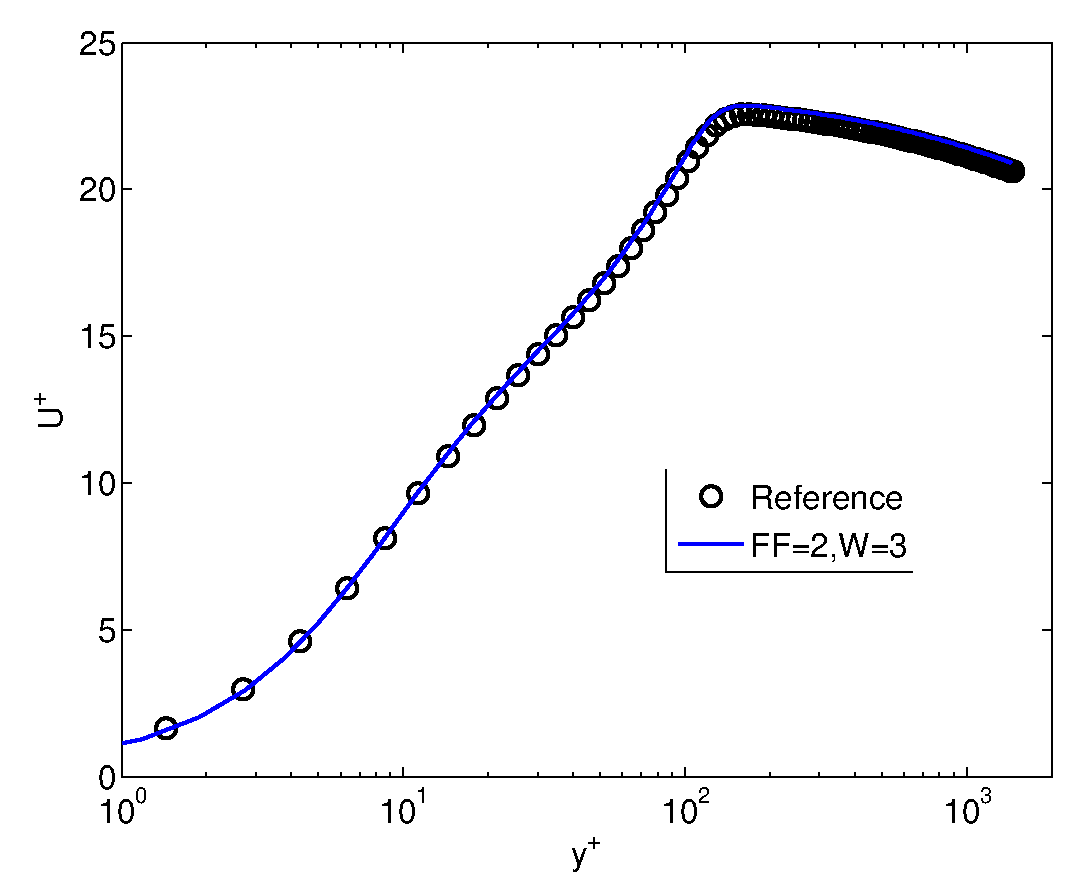
\includegraphics[width=0.9\columnwidth]{outflow_ff2w3_meanup}
		\caption{Mean flow}
		\label{fig:outflow_ff2w3_up}
	\end{subfigure}
	\begin{subfigure}[h]{0.49\textwidth}
		\centering
		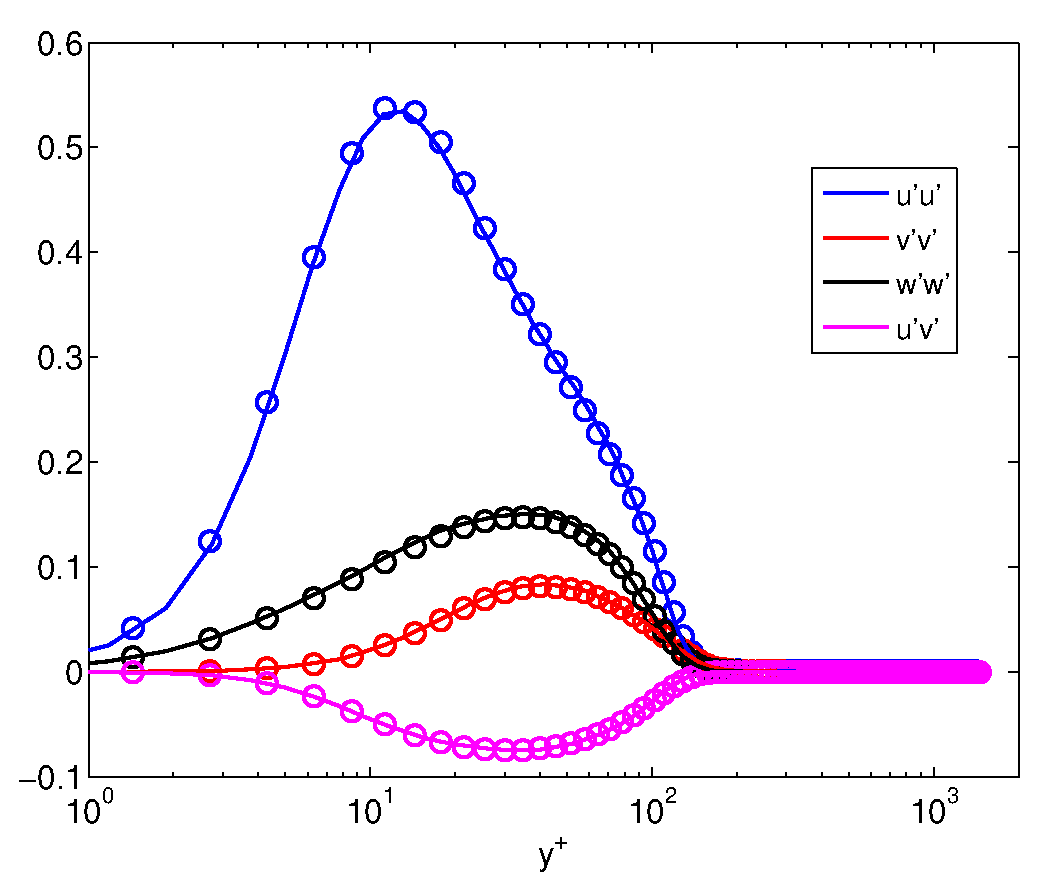
\includegraphics[width=0.9\columnwidth]{outflow_ff2w3_rs}
		\caption{Reynolds stresses}
		\label{fig:outflow_ff2w3_rs}
	\end{subfigure}
	\vspace{10pt}
	\caption{Comparison of wall-normal profiles of (a) mean tangential-flow and (b) Reynolds stresses for the case FF2W4.}
	\label{fig:outflow_ff2w3_u_rs}
\end{figure}
\begin{figure}
	\centering
	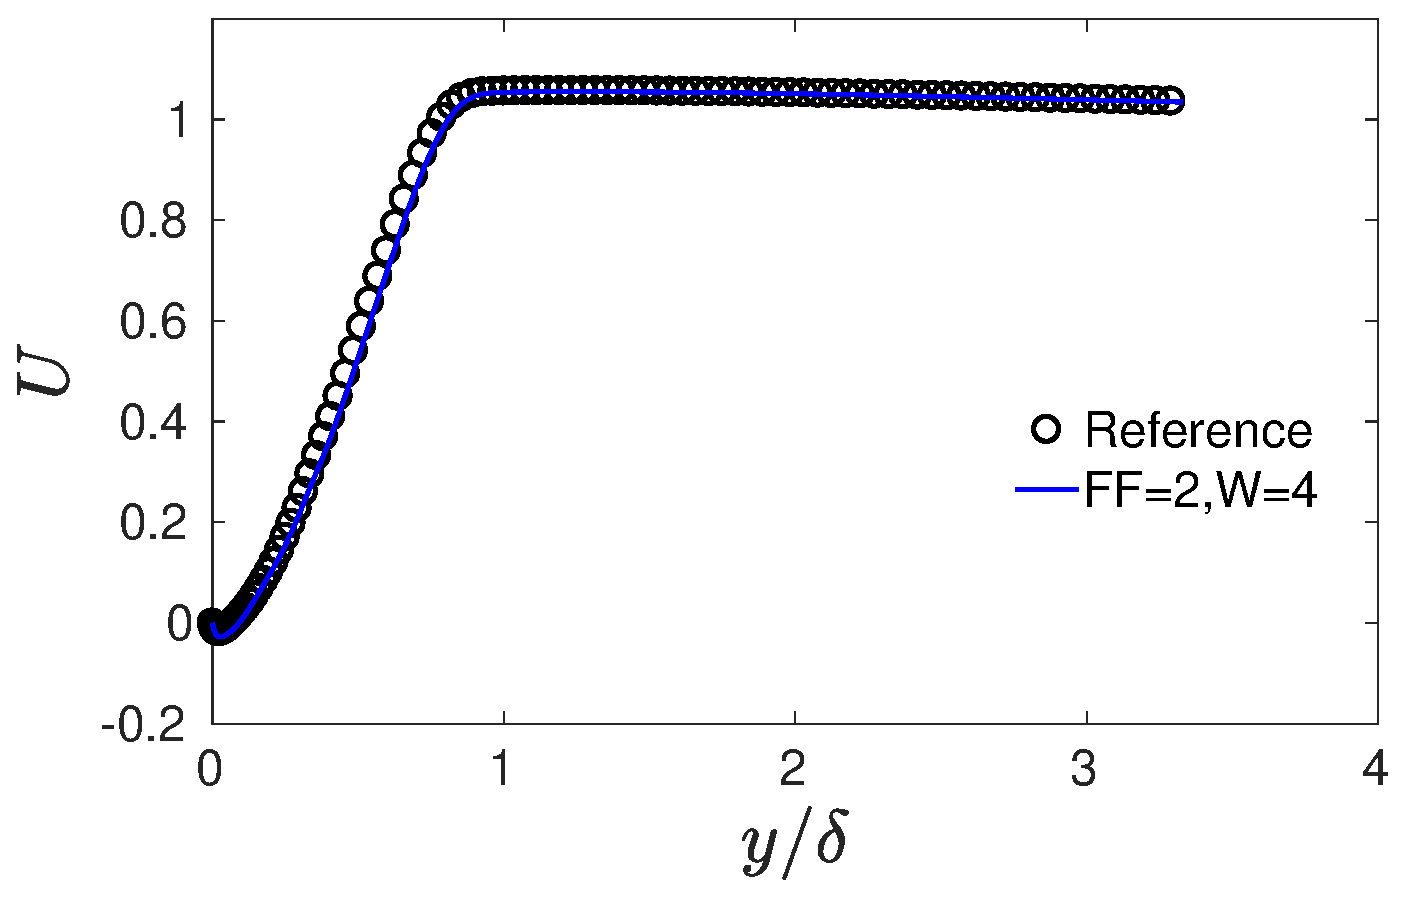
\includegraphics[width=0.5\columnwidth]{outflow_ff2w3_meanu_085}
	\vspace{5pt}
	\caption{Comparison of mean tangential-flow velocity profile in the separated region on the suction-side ($x/c=0.85$).}
	\label{fig:outflow_ff2w3_meanu_sep}
\end{figure}
Figure~\ref{fig:domain_ff2w3} shows a 2D x-y section of the truncated domain with figure~\ref{fig:grid_ff2w3} showing a close-up of the grid near the leading edge. The setup is very similar to the Reference case (figure~\ref{fig:domain_grid_reference}). Figure~\ref{fig:la2_ff2w3} shows the isocontours of flow structures identified by the $\lambda_{2}$ criterion, which look qualitatively similar to the ones seen in the reference case (figure~\ref{fig:la2_reference}).
\begin{figure}[h]
	\centering
	\begin{subfigure}[b]{0.49\textwidth}
		\centering
		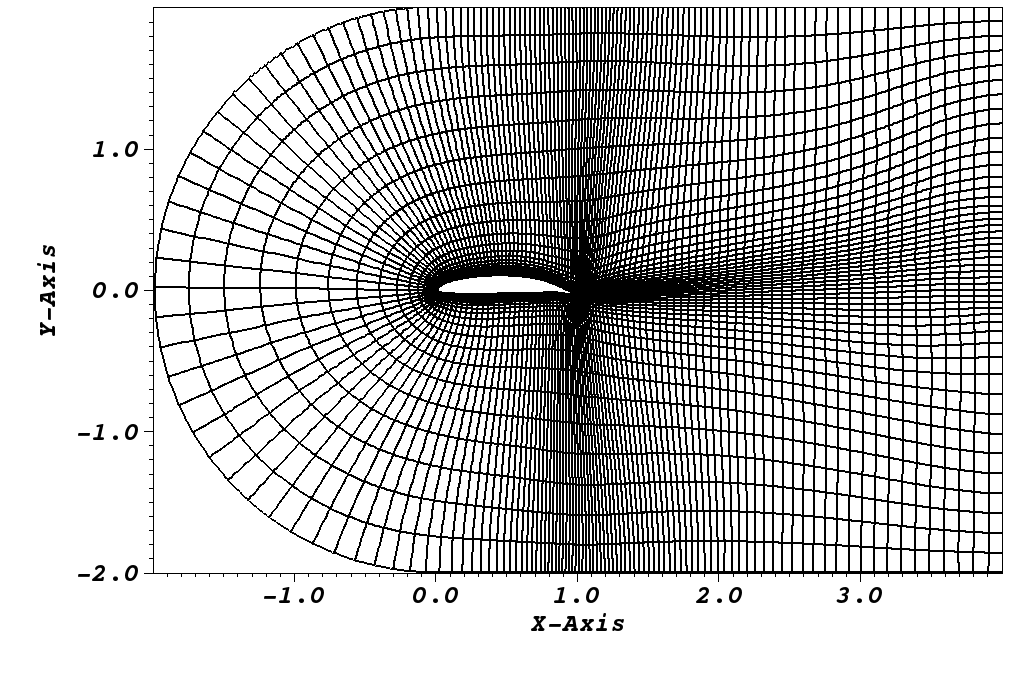
\includegraphics[width=1.0\columnwidth]{domain_ff2w3}
		\caption{Simulation domain}
		\label{fig:domain_ff2w3}
	\end{subfigure}
	\begin{subfigure}[b]{0.49\textwidth}
		\centering
		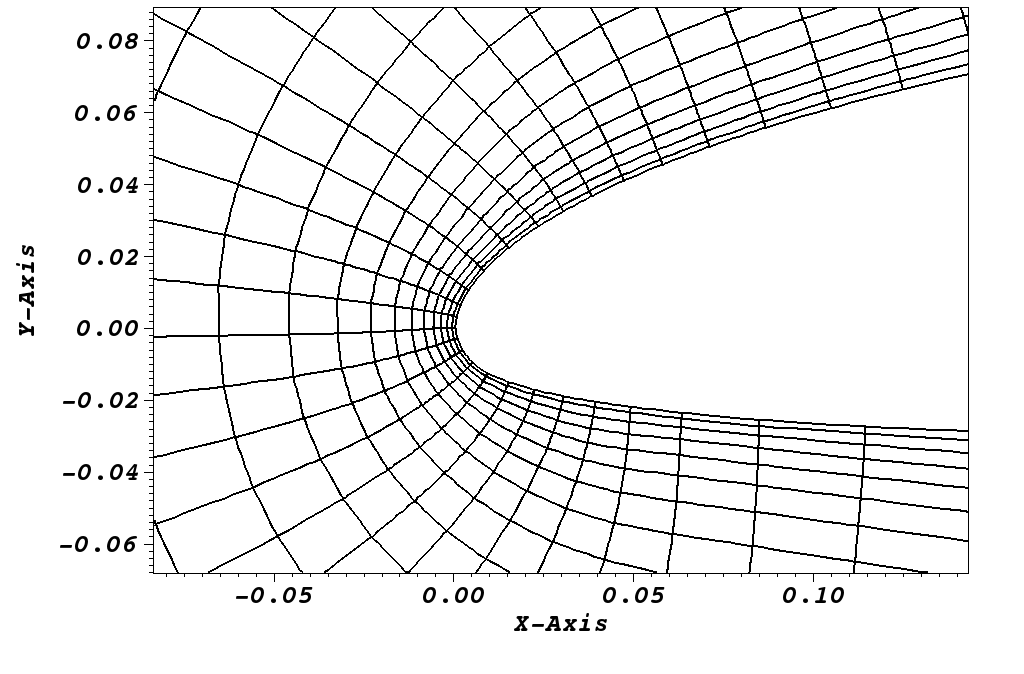
\includegraphics[width=1.0\columnwidth]{grid_ff2w3}
		\caption{Spectral-element grid}
		\label{fig:grid_ff2w3}
	\end{subfigure}
	\vspace{10pt}
	\caption{(a) Optimum truncated domain. (b) A close-up near the leading edge of the orthogonal and structured spectral-element grid. Domain is truncated such that the far-field is $2$ chords from the airfoil and the outflow is $4$ chords downstream from the leading-edge.}
	\label{fig:domain_grid_ff2w3}
\end{figure}

\begin{figure}
	\centering
	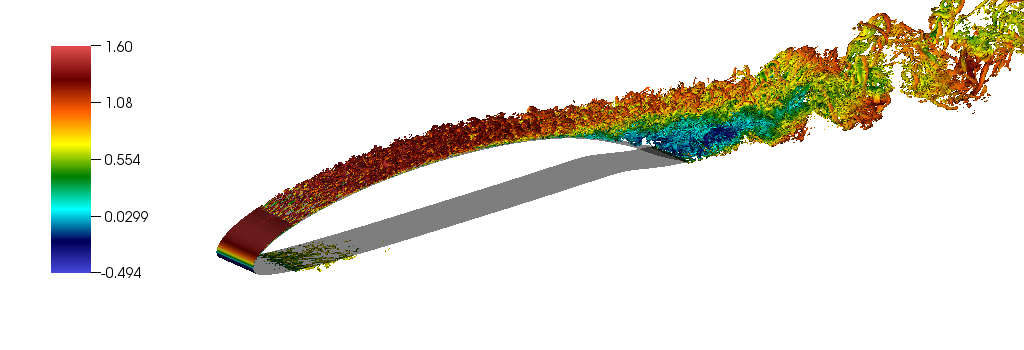
\includegraphics[width=0.9\textwidth,height=0.35\textwidth]{la2_ff2w3.png}
	\caption{Visualization of the instantaneous flow structures in the truncated domain. The flow structures are identified by the isocontours of the $\lambda_{2}$ criterion and are colored by streamwise velocity.}
	\label{fig:la2_ff2w3}
\end{figure}

%\FloatBarrier
\subsection{Summary}
Simulations of flow around a wing section with different domain sizes show that for a C-grid type mesh topology, flow distortion effects due to domain truncation and boundary conditions are minimized when the far-field boundary is two chords away from the airfoil leading-edge and the outflow boundary is four chords downstream of the leading-edge. The results are subject to the imposition of a RANS velocity field as Dirichlet boundary condition on the far-field boundaries and the energy-stabilized outflow boundary condition on the outlet boundaries of the simulation.
%===============================================================================

%\FloatBarrier
%\begin{footnotesize}
%\bibliography{scigenbibfile.Donald+Duck.Mickey+Mouse.Goofy+G.+Goof}\bibliographystyle{acm}
%\end{footnotesize}
%
%\end{document}
